\documentclass{ReportTemplate}
\usepackage{titlesec}
\usepackage[francais]{babel}
\usepackage[T1]{fontenc}
\title{CSEL}
\author{Macherel Rémy}
\date{\today}
\subtitle{Rapports des TP}
\subsubtitle{Git du projet : \href{https://github.com/Mathistis/csel-workspace}{https://github.com/Mathistis/csel-workspace}}
\location{Fribourg,}
\contact{remy.macherel@master.hes-so.ch}
\version{1.0}
\titlespacing*{\chapter}{0pt}{-60pt}{20pt}
\begin{document}

\maketitlepage

\newpage

\maketableofcontent

\medskip

\titleformat{\chapter}[display]
    {\Huge\bfseries}
    {}
    {0pt}
    {\thechapter.\ }
    

\chapter{Introduction}
Ce rapport décrit l'architecture ainsi que le développement et les
fonctionnalités du mini-projet réalisé lors du cours \textit{MA-CSEL} suivi lors
du semestre de printemps 2022 du master MSE. Ce projet consiste à mettre en
pratique les notions vues dans le cours par l'intermédiaire de l'implémentation
d'un gestionnaire de ventilateur pour le processeur de la cible. Notre cible
n'ayant pas de réel ventilateur, son fonctionnement sera simulé par le
clignotement d'une LED symbolisant un signal PWM pour piloter celui-ci ainsi qu'un écran
OLED affichant quelques valeurs importantes.\newline
Le but du travail est donc de concevoir une application permettant de simuler la
gestion de la vitesse de rotation d'un ventilateur en fonction de la température
du processeur. Les fonctionnalités suivantes seront donc implémentées:
\begin{itemize}
    \item Supervision de la température du processeur et la gestion de la
    vitesse de clignotement de la LED à l'aide d'un module noyau.
    \item Un daemon en espace utilisateur qui offrira des services pour une
    gestion manuelle et prendra en compte la gestion des appuis sur les boutons
    afin d'augmenter la vitesse de rotation, de la diminuer et de passer du mode
    manuel à automatique.\newline
    Ce daemon pourra également, à l'aide d'une interface IPC, communiquer avec
    une application de type \textit{CLI} pour la gestion du clignotement et du
    mode.
    \item Une application \textit{CLI} pour piloter le système via l'interface IPC.
\end{itemize}

\chapter{Architecture logicielle}
\begin{figure}[H]
    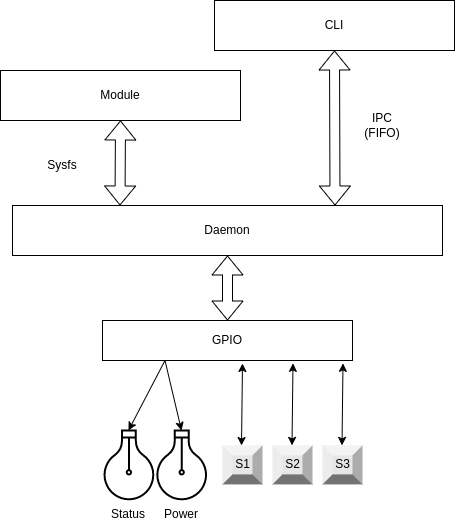
\includegraphics[width= \textwidth]{imageSources/Diagramme_Fonctions.drawio.png}
    \caption{Diagramme de principe de l'application}
    \label{fig:functionDiagram}
\end{figure}
\chapter{Conception du module}
Ce chapitre traite du développement du module noyau permettant de surveiller la
température du processeur ainsi que la gestion du clignotement de la LED status.
Ce module est dans le répertoire \textit{/sys/class/<mymodule>/...} et est composé de deux attributs:
\begin{itemize}
    \item is\_manu
    \item freq
\end{itemize}
Ces deux attributs sont représentés dans le userspace par des fichiers du sysfs.
Le but de ce module est de faire clignoter la LED en mode automatique ou en mode
manuel (si le mode manuel est actif, la valeur '1' est mise dans l'attribut
\textit{is\_manu}, si la valeur de l'attribut est '0', le mode automatique est activé). Le module implémente
un timer (\textit{<linux/timer.h>}) (voir fichiers \textit{timer\_controller.h
et .c}) qui est créé avec une fonction à exécuter lorsque son décompte est
terminé. Lorsque le temps est écoulé, cette fonction vérifie le mode actuel grâce à
l'attribut \textit{is\_manu} et si le
mode actuel est manuel, elle va regarder la fréquence inscrite dans le fichier
\textit{freq} puis calculer le prochain \textit{jiffies} correspondant à la
période de la fréquence de la manière suivante :
\usemintedstyle{vs}
\begin{minted}[linenos=False,frame=none]{c}
#define NEXT_JIFFIE_FROM_FREQ(freq) (jiffies + (HZ / freq))
\end{minted}
\textit{Remarque : Jiffies est une variable globale qui compte le nombre de
ticks qui se sont écoulés depuis le démarrage de la machine.}\newline
Il va ensuite changer l'état de la LED et réamorcer le timer.\newline
Pour le mode automatique, il va simplement lire la température du
microprocesseur et obtenir la fréquence correspondante (voir figure
\ref{fig:ledFrequencies}), puis écrire cette valeur dans le fichier freq et
réamorcer le timer.
\begin{figure}[H]
    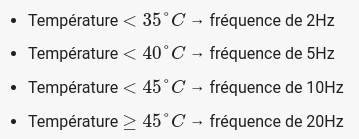
\includegraphics[width= \textwidth]{imageSources/Led_Frequencies.png}
    \caption{Fréquences pour la led en mode automatique}
    \label{fig:ledFrequencies}
\end{figure}
Dans le module, nous avons séparé les codes en deux parties, un fichier
\textit{controller.c} (avec son header file) qui représente une bibliothèque
permettant la gestion des modes du programme. Ce controller permet d'initialiser
les différents éléments utilisés dans le module (comme gpio, capteur de
température, timers, etc.), iil sert en quelque sorte à gérer les différents
composant du module noyau.\newline
Le deuxième fichier \textit{gpio.c} (également accompagné de son header file) permet quand à lui la gestion
des gpio ainsi que leur initialisation.\newline
Un autre code présent dans l'utilisation du module est le
\textit{temp\_controller}, celui-ci permet à l'aide de la bibliothèque
\textit{linux/thermal.h} de récupérer la température actuelle du
processeur.\newline
Dans le fichier \textit{skeleton.c} (le skeleton gère l'interface du module
noyau dans le sysfs), nous
appelons la fonction \textit{init\_controller} qui va permettre l'initialisation
des gpio, du timer ainsi que de la lecture de la température.\newline
Ce module va également créer et initialiser dans le sysfs les fichiers
nécessaires à la transmission de nos informations.\newline
Notre module étant de type \textit{class} il possède des attributs qui seront
stocké dans le sysfs sous \textit{/sys/class/<mod\_name>/...} et lors de la
déclaration des attributs du module (voir figure \ref{fig:sysfsInit}), on
définit deux variables statiques qui stockent la valeur des attributs au module ainsi que deux méthodes de lecture et
écriture qui permettront de gérer ces deux fichiers.
\begin{figure}[H]
    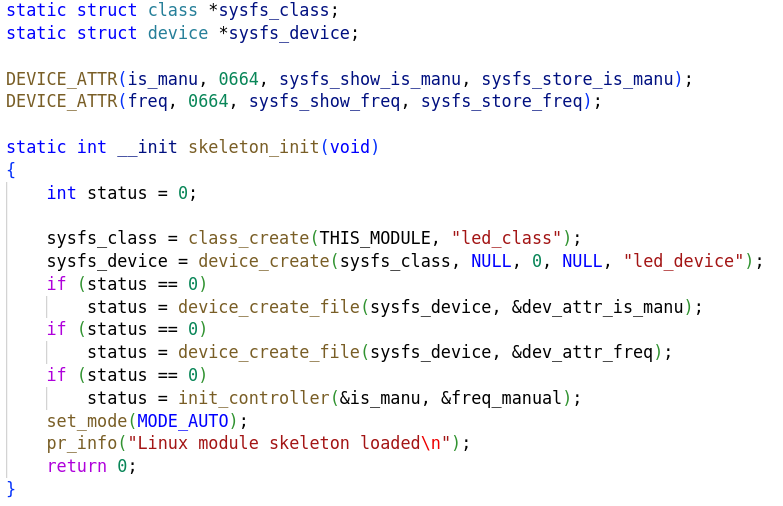
\includegraphics[width= \textwidth]{imageSources/Skeleton_Init.png}
    \caption{Création des fichiers nécessaires dans le sysfs}
    \label{fig:sysfsInit}
\end{figure}
Dans l'initialisation du module (figure \ref{fig:sysfsInit}), on se charge également de créer le device pour
le sysfs ainsi que les différents fichier qui nous servirons pour lire et écrire
nos valeurs.\newpage
Nous avons également dans ce module déclaré quelques fonctions permettant la
lecture ainsi que l'écriture des fichiers dans le sysfs.
\begin{figure}[H]
    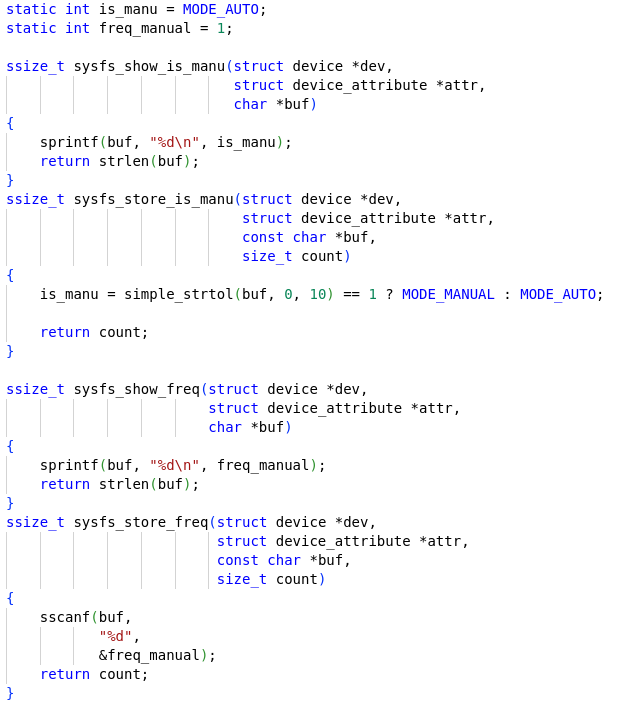
\includegraphics[width= \textwidth]{imageSources/Utility_Fct_Module.png}
    \caption{Fonctions de lecture/écriture des fichiers du sysfs}
    \label{fig:sysfsFunctions}
\end{figure}
On observe dans la figure \ref{fig:sysfsFunctions} que ces fonctions permettent
de lire et écrire les différents fichiers correspondant par exemple au mode
manuel ou l'affichage de la fréquence.\newpage
\section{Difficultés rencontrées sur le module}
Nous avons eu quelques soucis à fournir au début un code clair et bien séparé
c'est pourquoi nous avons opté pour la solution des controllers ainsi que des
fichiers séparés.\newline
Une autre difficulté fût de bien comprendre que \textit{DEVICE\_ATTR} est en
réalité une macro qui permet de créer plein de choses différentes concernant les
fichiers du sysfs et au premier abord nous n'avions pas pleinement conscience de
cela et avons eu un peu de peine à mettre en place ceci.
\chapter{Conception du daemon}
Ce chapitre traite du développement du deamon offrant les services permettant la
gestion de la fréquence ainsi que le choix du mode.\newline
Le daemon possède un timer qui lui permet de lire la température du processeur
grâce au module \textit{thermal} sité dans
\textit{/sys/class/thermal/thermal\_zone0/temp} ainsi que la fréquence dans notre
propre module. Cette lecture s'effectue toutes les 500ms (valeur choisie
arbitrairement pas nous-même), et lorsqu'il a pu obtenir ces valeurs, il va se
charger de mettre à jour l'affichage sur l'écran OLED. \newline
En plus de ce timer, il gère les boutons 1 à 3 afin de gérer le choix du mode
ainsi que la fréquence de la led lorsque le mode est manuel. Il se sert des
interruptions et de \textit{epoll} ainsi que du module \textit{GPIO} pour gérer
les boutons et ensuite écrit les valeurs dans le sysfs grâce au module
implémenté précédemment.\newline
Comme demandé dans la consigne, nous avons implémenté une FIFO afin de fournir
une interface IPC (Inter Process Communication) qui est également utilisée par
\textit{epoll}. Pour la mise en place de cette interface, nous avons défini un
simple protocole qui se présente de la manière suivante:\newline
Chaque message est de taille 8 bytes, en se basant sur la structure définie ci-dessous:
\begin{minted}[linenos=false,frame= none]{c}
struct cmd
{
    int cmd;
    int value;
}
\end{minted}
Les 4 premiers bytes sont utilisés pour la commande.
Actuellement seules deux commandes sont disponibles, \textit{SET\_MANUAL} pour
modifier \textit{is\_manual} et \textit{SET\_FREQ} pour modifier \textit{freq} en
mode manuel.
\begin{minted}[linenos=false,frame= none]{c}
#define FIFO_SET_MANUAL 0x14
#define FIFO_SET_FREQ 0x15
\end{minted}
La valeur 0x14 est donc utilisée pour modifier \textit{is\_manu} et la valeur
0x15 pour modifier \textit{freq}.\newline
Les 4 bytes suivants sont utilisés pour l'argument (ici \textit{value}). Pour le
choix du mode les valeurs sont 0 ou 1, pour la fréquence les valeurs sont entre
0 et \textit{MAX\_INT32}.\newline
\begin{figure}[H]
    \centering
    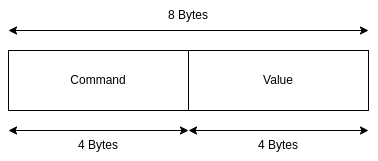
\includegraphics[width= 0.7\textwidth]{imageSources/Protocol.png}
    \caption{Protocole défini pour l'IPC}
    \label{fig:Protocol}
\end{figure}
Lorsqu'une commande arrive, \textit{epoll} réveille le daemon et la commande est
traitée.\newpage
Afin de créer le daemon, nous avons suivi la procédure vue en cours qui consiste
é créer un processus enfant puis de exit le processus parent afin d'avoir un
enfant détaché (daemon) qui va être rattaché au processus \textit{init} ceci est fait dans la fonction \textit{fork\_process()}.
\begin{figure}[H]
    \centering
    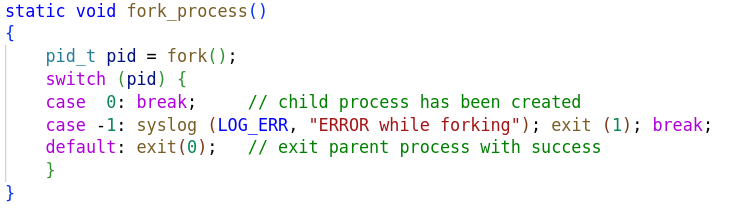
\includegraphics[width= 0.7\textwidth]{imageSources/fork_process.png}
    \caption{Fonction fork\_process}
    \label{fig:ForkProcess}
\end{figure}
On va ensuite créer une nouvelle session pour le nouveau processus avec le code
suivant:
\begin{minted}[linenos=false,frame= none]{c}
if (setsid() == -1) {
    syslog (LOG_ERR, "ERROR while creating new session"); 
    exit (1);
}
\end{minted}
Le processus sera ensuite session leader mais ce n'est pas encore notre but,
nous allons alors encore une fois utiliser \textit{fork\_process()} afin de
recréer un enfant et terminer son parent. une fois ceci fait, le processus démon
n'est plus session leader et n'a également plus accès au terminal.\newline
Nous avons ensuite déclaré la capture des signaux afin de les ignorer de la
manière suivante :
\begin{figure}[H]
    \centering
    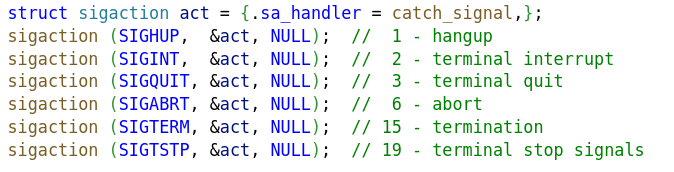
\includegraphics[width= \textwidth]{imageSources/signals_capture.png}
    \caption{Capture des signaux}
    \label{fig:SignalsCapture}
\end{figure}
\begin{figure}[H]
    \centering
    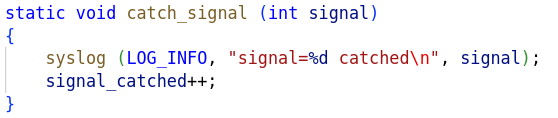
\includegraphics[width=\textwidth]{imageSources/catch_signal.png}
    \caption{Handler des signaux}
    \label{fig:CatchSignal}
\end{figure}
\newpage
Nous avons ensuite également mis à jour le masque pour la création de fichiers
avec la fonction \textit{umask()} et également fermé tous les descripteurs de
fichiers (\textit{close}), redirigé stdin,stdout,stderr vers \textit{/dev/null}
avec les fonctions \textit{open} et \textit{dup2}, puis enfin ouvert un fichier
de logging avec \textit{openlog()}.\newline
Pour la gestion du daemon, nous avons également opté pour un principe de
controller afin de gérer les différents évènements et actions du daemon. Après
la création du daemon, on utilise la fonction \textit{start\_controller()} qui va
se charger d'initialiser l'écran OLED, de créer les différents contextes
\textit{epoll} pour les boutons, initialiser la FIFO pour l'interface IPC, créer
un contrôle \textit{epoll} pour la FIFO et le timer (utilisé pour le
rafraichissement).\newline
Pour la gestion de ces différents évènements ainsi que les actions en découlant
et par soucis de propreté de code nous avons déclaré quelques header files et
fichiers dans lesquels nous avons défini différentes structures de données
facilitant la compréhension du code (voir dans
\textit{/workspace/src/miniprojet/daemon}).\newline
Chaque gpio correspondant aux boutons S1,S2,S3 est configuré dans le fichier
\textit{controller.c} à l'aide de la fonction \textit{open\_btn()} recupérée
d'un ancien TP. (\textit{/workspace/src/04\_system/silly\_led\_control.c}) Comme
dans cet ancien TP nous avons multiplexé les entrées (\textit{epoll}) afin
d'obtenir des évènements (bouton, timer, fifo) et pour chaque évènement nous
avons défini une structure avec un pointeur de fonction permettant d'exécuter le
code propre à chaque évènement.\newline
\section{Difficultées rencontrées sur le daemon}
Nous n'avons pas rencontré de difficultés particulières pour développer le
daemon si ce n'est le debug car en effet un daemon n'offre pas vraiment de
possibilités de print à l'écran (uniquement dans le fichier de logging créé mais
e n'est pas très pratique). C'est pourquoi nous avons tout d'abord développé son
fonctionnement comme si c'était une application cli classique et une fois
assurés du bon fonctionnement de l'application, nous avons instauré les
fonctions permettant de transformer celle-ci en daemon.\newline


\chapter{Application CLI}
Bien que rendue optionnelle sur la fin du projet, nous avons décidé
d'implémenter une application fournissant à l'utilisateur une interface CLI pour
la gestion du mode et le choix de la fréquence.\newline
\end{document}


